\documentclass[a4paper, 10pt]{article}
\usepackage[T1]{fontenc}
\usepackage[utf8]{inputenc}
\usepackage[slovene]{babel}
\usepackage{lmodern}
\usepackage{amsmath}
\usepackage{leftidx}
\usepackage{amssymb}
\usepackage{amsfonts}
\usepackage{graphicx}
\usepackage{wrapfig}
\usepackage{amsthm}
\usepackage{mathrsfs}
\usepackage{mathtools}
\usepackage{url}
\usepackage{subfigure}
\usepackage{multirow}
\usepackage{lipsum}
\usepackage{wrapfig}
\usepackage{tikz}
\usepackage[format=plain, font=small, labelfont=bf, textfont=it, justification=centerlast]{caption}
\usepackage{booktabs}
\usepackage{siunitx}
\usepackage{enumerate}
\usepackage{ulem}
\usepackage{cancel}
\usepackage{algorithm2e}

\newtheorem{trditev}{Trditev}
\newtheorem{izr}{Izrek}
\newtheorem{nal}{Naloga}
\newtheorem{posl}{Posledica}

\newcounter{defcount}
\newcounter{opombe}
\newcounter{zgledcount}

\newenvironment{opomba}{\begin{flushleft}\stepcounter{opombe}\textbf{Opomba \arabic{opombe}:}}{\hfill\end{flushleft}}
\setlength{\parindent}{0mm}

\newenvironment{zgled}{\begin{flushleft}\stepcounter{zgledcount}\textbf{Zgled \arabic{zgledcount}:}}{\hfill\end{flushleft}}
\setlength{\parindent}{0mm}

\newenvironment{definicija}{\begin{flushleft}\stepcounter{defcount}\textbf{Definicija \arabic{defcount}:}}{\hfill\end{flushleft}}
\setlength{\parindent}{0mm}

\newenvironment{resitev}{\begin{flushleft}\textit{Rešitev:}}{\hfill\end{flushleft}}
\setlength{\parindent}{0mm}

\newcommand{\abs}[1]{\ensuremath{\lvert #1 \rvert}}
\newcommand{\mth}[1]{\ensuremath{\mathbb{#1}}}
\newcommand{\R}{\mth{R}}
\newcommand{\Z}{\mth{Z}}
\newcommand{\N}{\mth{N}}
\newcommand{\No}{\mth{N}_0}
\newcommand{\C}{\mth{C}}
\newcommand{\Cc}{\ensuremath{\mathcal{C}}}
\newcommand{\Dd}{\ensuremath{\mathcal{D}}}
\newcommand{\Mu}{\mathcal{M}}
\newcommand{\sigalg}{$\sigma$-algebra~}
\newcommand{\Qu}{\mth{Q}_u}

\newcommand{\pojem}[1]{\emph{#1}}
\newcommand{\Ob}[1]{\mathcal{O}b({#1})}
\newcommand{\Mor}[2][ ]{\mathcal{M}or_{#1}({#2})}
\newcommand{\con}{\ensuremath{\mathscr{C}}}
\newcommand{\padex}[2]{\ensuremath{{#1}^{\underline{#2}}}}
\newcommand{\rastx}[2]{\ensuremath{{#1}^{\bar{#2}}}}
\newcommand{\map}[3]{\ensuremath{{#1}: {#2} \rightarrow {#3}}}
\newcommand{\pra}[3]{{#1}{\ast}({#2}) = {#3}}

\title{Osnove programiranja v diskretni matematiki\\ Zapiski predavanj}
\date{2023/24}
%===============================================================================
\begin{document}
	\maketitle
	\newpage
	\begin{abstract}
		\noindent Dokument vsebuje zapiske predavanj predmeta Osnove programiranja v diskretni matematiki profesorja Vesela v okviru študija prvega letnika magistrskega študija matematike na FNM.
	\end{abstract}
	\tableofcontents
	\newpage
	\section{Predstavitve grafov in onsnovni algoritmi nad njimi}
	\begin{definicija}
		\pojem{Graf} $G$ je sestavljen iz množice ogljišč $V(G)$ in množice povezav $E(G)$. Pišemo: $G = (V, E)$. Pri tem pogosto označimo \abs{V}$=n$ in \abs{E}$=m$.
		Za $v\in V(G)$ definiramo $d(v) =~\textit{število sosed vozlišča $v$ v grafu}~G$
	\end{definicija}
	\begin{zgled} \label{zgl:grafG} Poglejmo si naslednji graf in v tabeli določimo vsakemu vozlišču njegove sosede. $G:$
		
		
		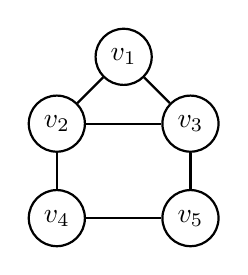
\begin{tikzpicture}[node distance = {12mm}, thick, main/.style = {draw, circle}]
			\node[main] (1) {$v_1$};
			\node[main] (2) [below left of=1] {$v_2$};
			\node[main] (3) [below right of=1] {$v_3$};
			\node[main] (4) [below of=2] {$v_4$};
			\node[main] (5) [below of=3] {$v_5$};
			
			\draw (1) -- (2);
			\draw (1) -- (3);
			\draw (2) -- (3);
			\draw (2) -- (4);
			\draw (3) -- (5);
			\draw (4) -- (5);
		\end{tikzpicture}
		
		\begin{table}[h!]
			\begin{tabular}{l|c|c|c|c|c|}
				Vozlišče & $v_1$ & $v_2$ & $v_3$ & $v_4$ & $v_5$ \\\hline
				Sosedi & $v_2, v_3$ & $v_1, v_3, v_4$ & $v_1, v_2, v_5$ & $v_2, v_5$ & $v_3, v_4$
			\end{tabular}
		\end{table}
	\end{zgled}
	Za predstavitev grafa imamo več možnosti. Prva možnost je matrika sosednosti, druga možnost (ki nas bo zanimala), pa so seznami sosedov. Seznami sosedov se izkažejo za bolj prostorsko varčne, saj matrika sosednosti tipično zavzame $O(n^2)$ mest, seznami sosedov pa manj. Koliko manj, je odvisno od načina implementacije.
	
	\subsection{Enostavni seznami sosedov}
	
	Sestavimo seznam $S$ vozlišč, tipično urejenih in oštevilčenih (npr $1$ predstavlja vozlišče $v_1$, $2$ vozlišče $v_2$ itd.). Nato sestavimo seznam sosedov $P$ tako, da po vrsti naštejemo sosede vozlišča $1$, nato vozlišča $2$, itd. Pri tem vsako vozlišče iz $S$ opremimo s kazalcem, ki kaže v $P$ na mesto, kjer se začnejo njegovi sosedi. 
	\begin{zgled}
		Predstavimo graf $G$ iz zgleda \ref{zgl:grafG} s pomočjo enostavnega seznama sosedov.
		\begin{table}[h!]
			$S$: \begin{tabular}{|c|c|c|c|c|}
				\hline
				$1$ & $2$ & $3$ & $4$ & $5$ \\\hline
			\end{tabular}
		\end{table}
		
		\begin{table}[h!]
			$P$: \begin{tabular}{|c|c||c|c|c||c|c|c||c|c||c|c|}
				\hline
				$2$ & $3$ & $1$ & $3$ & $4$ & $1$ & $2$ & $5$ & $2$ & $5$ & $3$ & $4$ \\\hline
			\end{tabular}
		\end{table}
	\end{zgled}
	Z $S_i$ označimo seznam sosedov vozlišča $v_i$. Seznam $S$ ima ravno $n$ mest, seznam $P$ pa $\sum_{i=1}^{n}d(v_i) = 2m$ mest. Prostorska zahtevnost enostavnih seznamov sosedov je torej $O(n + m)$, kar je po navadi res manj kot $O(n^2)$.
	\subsection{Razširjeni seznami sosedov}
	Najprej za vsako vozlišče $v_i$ sestavimo seznam sosedov $S_i$, v katerem vsakega od sosedov $v_i$ predstavimo s poljem $p$, ki je sestavljeno iz petih komponent: $p = (v_i, v_j, \&r, \&n, \&u)$. Pri tem je $v_i$ vozlišče, katerega sosede obravnavamo, $v_j$ ime soseda, $\&r$ kazalec, ki kaže na predhodnika $p$ v $S_i$, $\&n$ kazalec, ki kaže na naslednika $p$ v $S_i$ in $\&u$ kazalec, ki kaže na polje v seznamu $S_j$, ki predstavlja povezavo $v_iv_j$. Če je $p$ prvi v seznamu $S_i$ je $\&r = 0$, če je pa zadnji, je pa $\&n = 0$.
	
	\begin{zgled}
		\begin{table}[h!]
			\centering
			\begin{tabular}{|c|c|c|}
				Seznam & Ime polja & Polje \\\hline
				\multirow{2}{*}{$S_1$} & $a$ & $(v_1, v_2, 0, \&c, \&b)$ \\
				& $c$ & $(v_1, v_3, \&a, 0, \&d)$ \\\hline
				\multirow{3}{*}{$S_2$} & $b$ & $(v_2, v_1, 0, \&e, \&a)$ \\
				& $e$ & $(v_2, v_3, \&b, \&g, \&f)$ \\
				& $g$ & $(v_2, v_4, \&e, 0, \&h)$ \\\hline
				\multirow{3}{*}{$S_3$} & $d$ & $(v_3, v_1, 0, \&f, \&c)$ \\
				& $f$ & $(v_3, v_2, \&d, \&i, \&e)$ \\
				& $i$ & $(v_3, v_5, \&f, 0, \&j)$ \\\hline
				\multirow{2}{*}{$S_4$} & $h$ & $(v_4, v_2, 0, \&k, \&g)$ \\
				& $k$ & $(v_4, v_5, \&h, 0, \&l)$ \\\hline
				\multirow{2}{*}{$S_5$} & $j$ & $(v_5, v_3, 0, \&l, \&i)$ \\
				& $l$ & $(v_5, v_4, \&j, 0, \&k)$ \\\hline
			\end{tabular}
		\end{table}
	\end{zgled}
	Omenimo tukaj, da kadar grafu dodamo povezavo $v_iv_j$, to naredimo tako, da dodamo novo polje na začetek seznamov $S_i$ in $S_j$.
	\subsection{Časovna zahtevnost nekaterih operacij na grafih}
	Sedaj, ko smo uvedli različne sezname sosedov, lahko primerjamo časovno zahtevnost nekaterih klasičnih operacij na grafih.
	\begin{table}[h!]
		\centering
		\begin{tabular}{|c|c|c|}
			Operacija & Enostavni sez. & Razširjeni sez. \\\hline
			Preveri, če $G$ vsebuje povezavo $v_iv_j$ & $O(d(v_i))$ & $O(d(v_i))$ \\\hline
			Označi vse sosede vozlišča $v_i$ & $O(d(v_i))$ & $O(d(v_i))$ \\\hline
			Označi vse povezave & $O(m)$ & $O(m)$ \\\hline
			Dodaj povezavo $v_iv_j$ & $O(m)$ & $O(1)$ \\\hline
			Odstrani povezavo $v_iv_j$ & $O(m)$ & $O(d(v_i))$ \\\hline
			Odstrani vse povezave s krajiščem v $v_i$ & $O(m)$ & $O(d(v_i))$ \\\hline
		\end{tabular}
	\end{table}
	
	Izkaže se torej, da četudi imamo malenkost več dela z reprezentacijo grafov v razširjenih seznamih sosedov, s tem pridobimo na časovni zahtevnosti.
	
	\subsection{Urejanje seznamov sosedov}
	Za urejanje lahko, v splošnem, uporabimo algoritem z zahtevnostjo $O(k\log(k)$, kjer je $k$ število elementov seznama. Če to naredimo za vsak seznam dobimo: \begin{align*}
		\sum_{i=1}^{n} O(d(v_i)\log(d(v_i))) \leq \sum_{i=1}^{n} O(d(v_i)\log(n)) &= O(\log(n)\sum_{i=1}^{n}d(v_i)) \\
		&= O(m\log(n)) 
	\end{align*}
	To hitrost lahko torej pričakujemo pri enostavnih seznamih sosedov. Obstaja pa še hitrejši način, če si pomagamo z razširjenimi seznami sosedov. To naredimo tako, da upoštevamo, da je v vsakem polju seznama $S_i$ na v komponenti vozlišče $v_i$.
	Nove sezname gradimo tako, da se sprehajamo od seznama $S_n$, do $S_1$ in na vsakem koraku odstranimo polje $(v_i, v_j, \ldots)$ iz $S_i$. Nato odstranjenemu polju zamenjamo prvo in drugo komponento, da dobimo polje oblike $(v_j, v_i, \ldots)$ in to novo polje vstavimo na začetek novega seznama, ki ustreza vozlišču $v_j$. Algoritem še zapišemo bolj pregledno:
	\begin{algorithm}[h!]
		\DontPrintSemicolon
		\KwData{Razširjeni seznami sosedov $S_1,\ldots, S_n$}
		\KwResult{Urejeni razširjeni seznami sosedov $B_1,\ldots, B_n$}
		\SetAlgorithmName{Algoritem}
			~~Ustvari prazne razširjene sezname sosedov $B_1,\ldots, B_n$\;
			\For{i = n \text{downto} 1}{\While{$S_i\neq \emptyset$}{\Begin{Odstrani prvo polje~ $p=(v_i, v_j, \ldots)$iz $S_i$\; Dodaj $\acute{p} = (v_j, v_i, \ldots)$ na začetek $B_j$\;}}}
			\Return{$B_1, B_2, \ldots, B_n$}
			\caption{Algoritem za urejanje razširjenih seznamov sosedov}\label{alg:uredrazsezsos}
	\end{algorithm}
		
		Ta algoritem ima časovno zahtevnost $O(m)$, torej je hitrejši od algoritma na enostavnih seznamih sosedov, katerih urejanje je imelo časovno zahtevnost $O(m\log(n))$.
	\begin{definicija}
		Naj bosta $G$ in $H$ grafa. Bijekcija $\map{f}{V(G)}{V(H)}$ je \pojem{izomorfizem grafov}, če za poljuben par $u, v\in V(G)$ velja: $uv\in E(G) \iff f(u)f(v)\in E(H)$
	\end{definicija}
	Trenutno še ne poznamo algoritma, ki bi preveril, če sta dva grafa izomorfna, v polinomskem času. Lahko pa učinkovito preverimo, ali je dana bijekcija $\map{f}{V(G)}{V(H)}$ izomorfizem grafov, ali ne. Slednje nam pokaže naslednji izrek.
	\begin{izr}
		Za dana grafa $G$ in $H$ ter bijekcijo $\map{f}{V(G)}{V(H)}$ lahko v linearnem času preverimo, ali je $f$ izomorfizem.
	\end{izr}
	\begin{proof}
		Naj bodo $S_1, S_2, \ldots, S_n$ razširjeni seznami sosedov grafa $G$ in $C_1, C_2, \ldots, C_n$ razširjeni seznami sosedov grafa $H$. Najprej oblikujemo nove razširjene sezname sosedov $\acute{C}_1, \acute{C}_2, \ldots, \acute{C}_n$, kjer je $\acute{C}_i$ seznam, ki pripada $f(v_i); v_i\in V(G)$. Torej, $(f(v_i), f(v_j), \ldots)\in \acute{C}_i$.
		Sedaj z algoritmom \ref{alg:uredrazsezsos} za urejanje razširjenih seznamov sosedov uredimo $S_1, S_2, \ldots, S_n$ in $\acute{C}_1, \acute{C}_2, \ldots, \acute{C}_n$. Nato elemente seznamov $S_1, S_2, \ldots, S_n$ po vrsti zložimo v seznam $L_G$, elemente seznamov $\acute{C}_1, \acute{C}_2, \ldots, \acute{C}_n$ pa po vrsti v seznam $L_H$. Če je $f$ izomorfizem grafov, morata biti $L_G$ in $L_H$ identična v smislu, da za $\forall v_i \in L_G$ na enakem mestu v $L_H$ najdemo $f(v_i)$. Oba seznama uredimo v linearnem času $O(m))$, sestavljanje $L_G$ in $L_H$ tudi potrebuje $O(m)$ časa, torej časovna zahtevnost celotnega postopka $O(m)$.
	\end{proof}
	\section{Pregled grafa v širino}
	\begin{definicija}
		\pojem{Pot} v grafu $G$ je zaporedje paroma različnih vozlišč $v_1v_2\ldots v_k$, kjer za poljuben par zaporednih vozlišč iz poti velja $v_iv_{i+1} \in E(G) \forall i\in \{1, 2, \ldots, k\}$. Za vozlišči $u, v\in V(G)$ je \pojem{$u,v$-pot} pot, ki se začne v $u$ in konča v $v$. 
		\pojem{Razdalja} med vozlišči $u$ in $v$ je definirana s predpisom $d_G(u, v) = \min(\abs{p};~ p~\text{je $u, v$-pot})$. Pri tem je, za dano pot $p$, $\abs{p}$ dolžina poti $p$, torej število povezav v poti $p$.
	\end{definicija}
	Zapišimo sedaj algoritem za pregled grafa v širino.
		\begin{algorithm}[h!]
		\DontPrintSemicolon
		\KwData{Vozlišče $v\in V(G)$, razširjeni seznami sosedov $S_1,\ldots, S_n$ grafa $G$}
		\KwResult{Označitev $l$ množice vozlišč $V(G)$, kjer je $l(u) = d_G(v, u)$}
		\SetAlgorithmName{Algoritem}
		~~Pripravi vrsto (queue) $V = \{v\}$\;
		$l(v) = 0$\;
		\While{$V \neq \emptyset$}{\Begin{Odstrani $u$ iz začetka $V$\; \For{$w\in S_u$}{\If{$l(w)$ ni določen}{\Begin{$l(w)=l(u)+1$\; Vstavi $w$ na konec vrste $V$\;}}}}}
		\Return{Označitev $l$}
		\caption{Algoritem \pojem{BFS} za pregled grafa v širino}\label{alg:BFS}
	\end{algorithm}
	\begin{izr}
		Naj bo $C$ povezana komponenta grafa $G$ in naj bo $v\in V(C)$. Algoritem $BFS$ za vsako vozlišče $u\in V(C)$ določi $l(u) = d_G(v, u) = d_C(v, u)$ v času $O(\abs{E(C)})$
	\end{izr}
	\begin{proof}
		Najprej bomo dokazali pravilnost, nato pa še časovno zahtevnost.
		\begin{itemize}
			\item[Pravilnost:] Pravilnost bomo dokazali z indukcijo po $d(v, w) = i$. \begin{enumerate}
				\item[$i = 0:$] v tem primeru je $d(v, w) = 0$, kar je možno le, ko je $w = v$. Sledi, da je $l(w) = 0 = l(v)$. V vrsto $V$ algoritma prihajajo vozlišča na eni strani in odhajajo na drugi. Ker $l$ povečujemo, dobimo naraščajoče zaporedje in sosednji vozlišči se razlikujeta za največ $1$.
				\item[$i>0:$] Denimo, da izrek velja za vsa vozlišča $v, u \in V(C)$, za katera je $d(v, u)\leq i$. Opazujemo $w\in V$ za katerega je $d(v, w) = i+1$. Za tak $w$ obstaja nek $u_0\in V(C)$, da je $d(v, u_0) = i$ in $u_0w\in E(C)$. Po indukcijski predpostavki je potem $l(u_0)=i$, to oznako pa smo dobili od nekega vozlišča, ki je od $v$ oddaljeno za $i-1$. Oznake vozlišč na razdalji $i$ dobimo tako, da najprej sprocesiramo vozlišča, ki so na razdalji $i-1$, teh vozlišč pa na tej točki ni več v $V$. V vrsti $V$ so torej samo vozlišča, ki so od $v$ oddaljene $i$. Potem je pa $l(w) = i+1$.
			\end{enumerate}
			\item[Čas. zaht.:] Telo \pojem{for} zanke se izvede $2\abs{E(C)}$-krat z zahtevnostjo $O(1)$, torej je skupna zahtevnost $(\abs{E(C)})$.
		\end{itemize}
	\end{proof}
	\begin{definicija}
		\pojem{Matrika razdalj} $D$ grafa $G$ je matrika dimenzije $\abs{V(G)}\times\abs{V(G)}$ za katero velja $d_{i, j} = d_G(v_i, v_j) \forall i,j\in \{1, 2, \ldots, \abs{V(G)}\}$.
	\end{definicija}
	
	\begin{posl}
		Naj bo $G$ graf in $\abs{V(G)} = n$ ter $\abs{E(G)} = m$. Tedaj velja: \begin{enumerate}[i)]
			\item Povezane komponente $G$ lahko poiščemo v času $O(n+m)$
			\item Matriko razdalj grafa $G$ lahko poiščemo v času $O(mn)$
		\end{enumerate}
	\end{posl}
	\begin{proof}
		\begin{enumerate}[i)]
			\item Sprehodimo se po vseh vozliščih grafa in za vsako vozlišče z nedoločenim $l$ poženemo algoritem \ref{alg:BFS}. Za vsako povezano komponento $C$ grafa $G$ nas to stane $O(\abs{E(C)})$, torej je skupna časovna zahtevnost za cel graf $G$ enaka $O(m)$. Če ima graf manj od $n$ povezav, je vseeno treba obiskati vsa vozlišča. Skupen čas celotnega postopka je torej $O(m + n)$.
			\item Za vsako izmed $n$ vozlišč poženemo algoritem \ref{alg:BFS}. Vsaka izvedba tega algoritma ima zahtevnost $O(m)$, izvedb pa je $n$, torej je zahtevnost celotnega postopka $O(mn)$
		\end{enumerate}
	\end{proof}
	\begin{zgled}
		Vrnimo se k grafu $G$ iz zgleda \ref{zgl:grafG} in mu določimo tabelo označitev za začetno točko $v = 1$.
		\begin{table}[h!]
			\centering
			\begin{tabular}{c|c|c|c|c|c|c}
				$u$ & $v$ & $l_1$ & $l_2$ & $l_3$ & $l_4$ & $l_5$ \\\hline
				& $1$ & $0$ & & & & \\\hline
				$1$ & $2, 3$ & & $1$ & $1$ & & \\\hline
				$2$ & $3, 4$ & & & & $2$ & \\\hline
				$3$ & $1, 5$ & & & & & $2$\\\hline
				$4$ & $2, 5$ & & & & & \\\hline
				$5$ & $3, 4$ & & & & & \\
			\end{tabular}
		\end{table}
	\end{zgled}
	Če poženemo \pojem{BFS} algoritem za neko začetno vozlišče $v\in V(G)$ lahko $V(G)$ razbijemo na množice $L_0, L_1,\ldots$, kjer je $L_i =\{u\in V(G) ;~d(v, u) = i\}$. \begin{definicija}
		Naj bo $G$ graf in $v\in V(G)$. Če je $u\in L_i$ in $uw\in E(G)$ in \begin{itemize}
			\item Če je $w\in L_{i-1}$, pravimo, da je $uw$ \pojem{povezava navzgor}
			\item Če je $w\in L_{i+1}$, pravimo, da je $uw$ \pojem{povezava navzdol}
			\item Če je $w\in L_{i}$, pravimo, da je $uw$ \pojem{povezava povprek}
		\end{itemize}
	\end{definicija}
	Za povezan graf $G$ lahko skonstruiramo t.~i.~\pojem{$BFS$-drevo} s korenom v $v\in V(G)$. Za $BFS$-drevo $T$ s korenom $v\in V(G)$ velja: $D_T(v, u) = d_G(v, u)~\forall u\in V(T)\subseteq V(G)$. Če je $V(T) = V(G)$ se spomnimo, da pravimo, da je $T$ \pojem{vpeti podgraf} grafa $G$.
	\begin{definicija}
		Graf $G$ je \pojem{dvodelni graf}, če obstaja \pojem{razbitje} $V(G) = (X, Y)$, tako da za vsako povezavo iz $E(G)$ velja, da ima eno krajišče v $X$ in drugo krajišče v $Y$
	\end{definicija}
	\begin{trditev}
		\label{trd:dvodelgraf1}
		Graf $G$ je dvodelen $\iff$ $G$ ne vsebuje lihega cikla
	\end{trditev}
	\begin{trditev}
		Graf $G$ je dvodelen $\iff$ $G$ ne vsebuje povezave povprek za $BFS$ označitev, ki se začne v poljubnem $v\in V(G)$
	\end{trditev}
	\begin{proof}
		\begin{itemize}
			\item[$\Rightarrow:)$] Denimo, da obstaja neka povezava povprek $uw\in E(G)$ za neki vozlišči $u\in X$ in $w\in Y$, kjer je $(X, Y)$ razbitje $G$. Potem obstaja tak $i\in \{1, 2, \ldots, n\}$, da je $d(v, u) = i =d(v, w)$. Ker sta $X$ in $Y$ povezani, graf $G$ potem vsebuje en cikel dolžine $2i + 1$, to je pa protislovno s tem, da je $G$ dvodelen po trditvi \ref{trd:dvodelgraf1}.
			\item[$\Leftarrow:)$] Za vozlišče $v\in V(G)$ izvedemo $BFS$ algoritem in definiramo $X = \bigcup_{i = 0} L_{2i}$ ter $Y = \bigcup_{i = 0}L_{2i+1}$. Očitno je $X\cup Y = G$ in $X\cap Y = \emptyset$, torej je $(X, Y)$ razbitje $G$. Ker $G$ nima povezav povprek za $u\in L_i in uw\in E(G)$ velja, da je $w\in L_{i-1}$ ali pa je $w\in L_{i+1}$. Torej, če je $u\in L_i \subseteq X$, je potem $w\in Y$ in obratno, če je $u\in L_i \subseteq Y$, je $w\in X$. Za vsako povezavo $uw\in E(G)$ je potem eno krajišče iz $X$ in drugo iz $Y$. Potem je pa $G$ dvodelni graf.
		\end{itemize}
	\end{proof}
	\begin{trditev}
		Dvodelne grafe lahko prepoznamo v linearnem času.
	\end{trditev}
	\begin{proof}
		Vemo, da lahko za vsak $v\in V(G)$ algoritem $BFS$ izvedemo v linearnem času. Naj bo torej $v\in V(G)$ poljubno vozlišče in se sprehodimo po vseh povezavah. Po prejšnji trditvi bo potem $G$ dvodelen $\iff$ vsak par zaporednih krajišč ima različni oznaki.
	\end{proof}
\end{document}